%! alt A kite-shaped convex quadrilateral ABCD with P, Q, R, S on sides AB, BC, CD, DA. The segments PR and QS cross at O and split ABCD into four quadrilaterals, and in each the diagonal through O is perpendicular to the opposite diagonal: OA is perpendicular to PS, OB to PQ, OC to QR and OD to RS, marked with right angles. The circle through P, Q, R and S is dashed. Adapted from Beyond the Incenter, Problem 96.
%! after_paragraph 0
%! scale 1
% The shared preamble of every Cevian figure. pipeline/figures turns these colours into theme-aware paint,
% and refuses any other colour, so draw only with them:
%   figink (lines and labels), figaux (construction lines), figaccent (the object the argument turns on),
%   figtint and figaccenttint (light fills).
\documentclass[border=1.5pt]{standalone}
\usepackage{tkz-euclide}
\definecolor{figink}{RGB}{0,0,0}
\definecolor{figaux}{RGB}{85,85,85}
\definecolor{figaccent}{RGB}{192,57,43}
\definecolor{figtint}{RGB}{221,221,221}
\definecolor{figaccenttint}{RGB}{245,213,208}
% tkz-euclide's defaults draw circles, compasses and marks in 50% grey and fill points with a tint.
\makeatletter
\def\tkz@otherlinecolor{figink}
\def\tkz@euc@circlecolor{figink}
\def\tkz@euc@compasscolor{figink}
\def\tkz@euc@mkcolor{figink}
\def\tkz@mk@fill{figink}
\def\tkz@euc@pointfillcolor{figink}
\makeatother
\tkzSetUpLine[color=figink,line width=.7pt]
\tkzSetUpArc[color=figink,line width=.7pt]
\tkzSetUpCompass[color=figink,line width=.5pt]
\tkzSetUpPoint[color=figink,fill=figink,size=3.1pt]
\tikzset{
  every picture/.style={line cap=round,line join=round,color=figink},
  circle style/.append style={color=figink,line width=.7pt},
  aux/.style={color=figaux,line width=.45pt,dash pattern=on 2.6pt off 2pt},
  key/.style={color=figaccent,line width=1pt},
  mk/.style={color=figink,line width=.5pt},
  lbl/.style={color=figink,inner sep=2.2pt},
  len/.style={color=figink,inner sep=1.5pt,font=\small},
}

\begin{document}
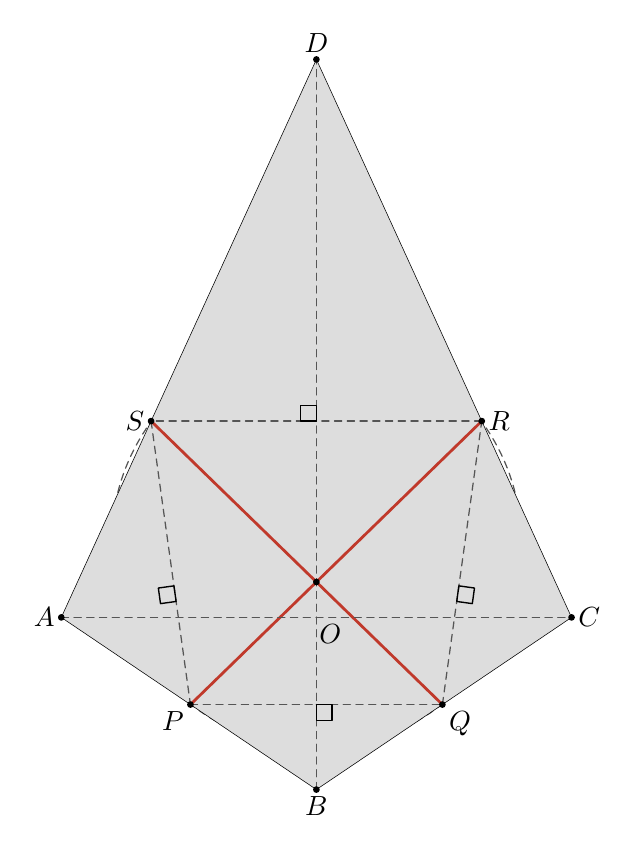
\begin{tikzpicture}
\tkzDefPoint(-1.6000000,-1.5000000){P} %! P = (-8/5, -3/2)
\tkzDefPoint(1.6000000,-1.5000000){Q} %! Q = (8/5, -3/2)
\tkzDefPoint(2.1000000,2.1000000){R} %! R = (21/10, 21/10)
\tkzDefPoint(-2.1000000,2.1000000){S} %! S = (-21/10, 21/10)
\tkzDefPoint(0.0,0.056756757){O} %! O = meet(P, R, Q, S)
\tkzDefPoint(0.0,0.55694444){Z} %! Z = circumcentre(P, Q, R)
%! let s = 9/10
\tkzDefPoint(-3.2400000,-0.39324324){A} %! A = (x(O) - s*(y(S) - y(P)), y(O) + s*(x(S) - x(P)))
\tkzDefPoint(3.2400000,-0.39324324){C} %! C = (-x(A), y(A))
\tkzDefPoint(0.0,-2.5797627){B} %! B = meet(A, P, O, shift(O, 0, 1))
\tkzDefPoint(0.0,6.6928165){D} %! D = meet(C, R, O, shift(O, 0, 1))
\tkzDefPoint(-1.7818442,-0.19072161){E} %! E = meet(A, O, P, S)
\tkzDefPoint(0.0,-1.5000000){F} %! F = meet(B, O, P, Q)
\tkzDefPoint(1.7818442,-0.19072161){G} %! G = meet(C, O, Q, R)
\tkzDefPoint(0.0,2.1000000){H} %! H = meet(D, O, R, S)
%! fact concyclic(P, Q, R, S)
%! fact on_segment(P, A, B)
%! fact on_segment(Q, B, C)
%! fact on_segment(R, C, D)
%! fact on_segment(S, D, A)
%! fact perp(A, O, P, S)
%! fact perp(B, O, P, Q)
%! fact perp(C, O, Q, R)
%! fact perp(D, O, R, S)
\tkzDrawCircle[aux](Z,P)
\tkzFillPolygon[color=figtint](A,B,C,D)
\tkzDrawPolygon(A,B,C,D)
\tkzDrawSegments[aux](P,Q Q,R R,S S,P)
\tkzDrawSegments[key](P,R Q,S)
\tkzDrawSegments[aux](A,C B,D)
\tkzMarkRightAngle[size=.2,mk](A,E,S)
\tkzMarkRightAngle[size=.2,mk](B,F,Q)
\tkzMarkRightAngle[size=.2,mk](C,G,R)
\tkzMarkRightAngle[size=.2,mk](D,H,S)
\tkzDrawPoints(A,B,C,D,P,Q,R,S,O)
\tkzLabelPoint[left,lbl](A){$A$}
\tkzLabelPoint[below,lbl](B){$B$}
\tkzLabelPoint[right,lbl](C){$C$}
\tkzLabelPoint[above,lbl](D){$D$}
\tkzLabelPoint[below left,lbl](P){$P$}
\tkzLabelPoint[below right,lbl](Q){$Q$}
\tkzLabelPoint[right,lbl](R){$R$}
\tkzLabelPoint[left,lbl](S){$S$}
\tkzLabelPoint[xshift=5pt,yshift=-13pt,lbl](O){$O$}
\end{tikzpicture}
\end{document}
